%!TEX root = ../thesis.tex
\chapter{Results}
\label{chap:Results}
In this Chapter I characterise the methodology detailed in Chapter  \ref{chap:BHM} and then I applied it to the Pleiades DANCe DR2 data set (Sect. \ref{sect:DR2}). To characterise the methodology as a classifier, I measure its precision and accuracy when applied on synthetic data where the true members of the cluster are known. With this characterisation, I am able to obtain an optimal probability threshold, but only for classification purposes. Afterwards, I apply the methodology to the Pleiades DANCe RDR2 and I find the candidate members of the cluster using the optimal probability threshold. Then, I compare these candidate members with those found by previous studies.

Later, I analyse the main results of this work, those that fulfil the objective: the statistical distributions that characterise of the cluster population. Then, l give the details of the spatial, velocity, luminosity and mass distributions. Finally, I end this Chapter describing the physical scenario of the evolution of the mass distribution of the Pleiades by comparing it with other mass distribution of younger and older clusters.

\section{Performance of the classifier}
\label{sect:classifier}
As mentioned earlier, the main objective of the methodology of the BHM is the statistical characterisation of the NYOC populations. However, as a by product, it also obtains the individual membership probability distributions of the objects comprising the data set. These membership probability distributions, together with a probability threshold, allow a direct classification of the objects into cluster and field members.  The classification resulting from this procedure, as any other measured property, has an uncertainty. By evaluating this uncertainty under the results of synthetic data (in which the true members are known) we are able to measure the accuracy and precision of the classification process as a function of the probability threshold used. This section explains how an objective probability threshold can be found by maximising the accuracy of the classifier. 

To measure the accuracy of our classifier, I test it over synthetic data sets that resemble the real RDR2 (Section \ref{sect:RDR2}). An ideal test to our classifier will be to apply it over well known dataset in which tags of cluster and field members were already present. However, if we may have access to these tags, a classifier may not be needed. The Pleiades cluster being one of the most studied cluster in history, it is the NYOC with most of these tags (see Section \ref{sect:memberscomparison}). This is one the reasons for which we decided to benchmark our methodology on it. In spite of the large number of candidate members for the Pleiades clusters, the synthetic data and its true tags are still needed. The reasons are the following. First, the list of candidate members provided by the literature is not infallible. We can never be sure that this list is complete and unpolluted. Here it is important to note that the astrophysical domain of the phenomenon marks a very important distinction with common supervised classification methods. A perfect and real training set is not available. It must be created from simulations. Second, even if the most probable candidate members from the literature were used as a training set \cite[as done for example by][]{Sarro2014} the very faint end of the magnitude distribution (represented by brown-dwarfs) is still a \emph{terra ignota} where candidate members are scarce or not even exist. 

Thus, to overcome the problem of the true tags, we decided to create synthetic data sets. These synthetic true tags, and therefore, the results obtained from them relay under the assumption that our cluster and field models resemble the real data. I am aware that these models are far from perfect, but so far this assumption provides the best option. Although this assumption enable us to quantify the internal consistence (precision and accuracy) of our classifier, it does not give any indication about possible biases in the model. To explore this possibility, in the next Section, I compare our real data classification results with those of the literature.

The random nature of the synthetic data sets demands the repetition of the data sets and results. This repetitions avoid any bias caused by excursions of the random number generator (bad luck), and more importantly, they allow us to compute the uncertainty in the accuracy and precision of the classifier. As explained before, the methodology presented in this work is computing demanding. Thus, to be able to repeat at least five times the results of the synthetic data sets, we further reduce the data set size. The inference process in a data set of $10^4$ objects demands almost week of computing time. Thus, we decided that such data set provided a good compromise between computing time and number of objects. Furthermore, to provide a better estimate of the contamination rate on the results over the real RDR2 data set (the one with the $10^5$ objects) we choose to work with the $10^4$ objects with high membership probability according to \citet{Bouy2015}. Since this sample is relatively more entangled with the cluster than that of the RDR2, we assume that the contamination rate we measure on this sample will be comparable or even higher than that hypothetically obtained over the $10^5$ RDR2. 

Briefly, to create the synthetic data set, the procedure is the following. First, using the methodology of the previous Chapter, I obtain a sample of the posterior distribution of the parameters in the model given the $10^4$ real data set. Then, I choose the particle with highest posterior probability as the MAP estimate of the posterior distribution. Using this particle positions in the parametric space, I generate five synthetic data sets of $10^4$ objects each. Then, I tag these objects according to their parent population: cluster or field. Afterwards, using the vector of synthetic values of each object, I assign their uncertainties and missing value entries (more details  below).

Finally, I run the methodology over the five synthetic data sets, and obtain a sample of the individual membership probability distributions of each synthetic object. Then, I compare the true tags with the measured ones as function of the probability threshold. 

To further test the performance of the classifier, I apply it on a synthetic data set in two different cases. In the first case the data set is one of the five synthetic ones. Thus it contains objects with missing value entries in their vector of observables.  In the second case the data set is the same as in the previous case, but this time all the objects have fully observed vectors (i.e. do not have missing value entries). The comparison of the results rendered by these two cases allows us to quantify the impact of missing values. 

Objects in the Pleiades DANCe DR2  have full observed proper motions vectors. Since missing values appear only in the photometric vectors, in synthetic data sets I only include missing values in the photometry. Only $\sim1\%$ of the objects in the RDR2 have full observed vectors (i.e. no missing value entries). Furthermore, the distribution of missing entries is not random and depends on the magnitudes of the objects (see Fig. \ref{fig:NAsKs}). Therefore, to better reproduce this distribution in the synthetic data sets, for each synthetic datum, I use the mask of missing entries of one of its closer neighbours in the real data set. Here, distance is measured in the euclidean sense. If I were to use the missing value mask of the nearest neighbour in the real data set, then I will obtain a biased sample in which objects with full observed vectors (with no missing entries) will be underestimated. This is the inevitable consequence of the fact that euclidean distances measured in subspaces, which result from removing the dimensions of the missing entries, are small, or at most equal, than those measured in the complete space. 

To reproduce the mask of missing entries, I choose from among those masks of the closer neighbours in the available CMDs: $\{K_s,J-K_s\},\{J,J-H\},\{K_s,H-K_s\},\{J,Y-J\},\{K_s,i-K_s\}$. These CMD are formed with the bands and colours of the magnitudes with fewer missing values, in decreasing order (see Table \ref{tab:DR2properties}).  The mask of missing entries to reproduce in the synthetic objects is chosen as follows. First, for each CMD subspace I find the set of objects, from the real data set, with fully observed entries, I call it $C_{or,i}$ and its fraction from the total, $f_r$. Then, I take a random sample from the synthetic data whose fraction, $f_s$ equals $f_r$. For objects in this sample I assign the missing value pattern of the nearest neighbour in $C_{or,i}$. I repeat this procedure for the rest of the CMDs. In this way, the synthetic data sets have fractions of objects with and without missing entries, similar to those of the objects in the real data set.

To assign uncertainties I proceed as follows. For uncertainties in the proper motions I use those of the nearest neighbour from the real data set. If I were to use the nearest neighbour scheme for uncertainties in the photometry, then I will obtain biased results. These uncertainties will be biased towards those of the less precise measurements. Again, this is a consequence of the missing entries in the observable vectors. The euclidean metric results in the preferential choosing of objects with missing values. These missing values occur mostly at the faint end, where uncertainties are larger. Therefore, these uncertainties will be biased towards these larger values. To avoid this issue, I fit 8th degree Chebyshev polynomials to the uncertainties as a function of the magnitudes. Then, I use these polynomials to establish the photometric uncertainties of the synthetic data sets.

Once the synthetic data sets were created I run the methodology on each of them and recover the membership probability distribution of each object. Then, I classify each object as cluster or field member. To classify an object as a cluster member, the mode of its cluster membership probability distribution must be higher than the probability threshold. Otherwise it is classified as a field object. 

The classifier performance was measured by counting the true positives (TP, cluster members correctly classified), true negatives (TN, field members correctly classified), false positives (FP, field members classified as cluster members) and false negatives (FN, cluster members classified as field members) recoveries as a function of the probability threshold. With them I calculate the following quantities: the true positive rate (TPR), which is the ratio of true positives over the sum of true positives plus false negatives, the contamination rate (CR), which is the ratio of false positives over the sum of false positives plus true positives, the precision or positive predictive value (PPV), which is the ratio of true positives over the sum of true positives plus false positives, and, the accuracy (ACC), which is the ratio of the sum of true positives plus true negative over the sum of true and false positives and negatives. 

These are,
\begin{align}
TPR &= \frac{TP}{TP+FN} \nonumber \\
CR   &= \frac{FP}{FP+TP} \nonumber \\
PPV &= \frac{TP}{TP+FP} \nonumber \\
ACC &= \frac{TP+TN}{TN+FN+TP+FP},\nonumber
\end{align}
which are defined at each probability threshold. I use the results of the five synthetic data sets to quantify the uncertainties of the previous quantities. 

In Fig. \ref{fig:TPR-CR}, I show the mean and uncertainty of the TPR and CR measured on the five synthetic data sets. The uncertainty is represented by the maximum deviation from the mean. Also, this Figure shows the TPR and CR measured on a synthetic data set with fully observed objects (i.e. objects with non missing entries). As this Figure shows, the missing values have a negative impact in our classification. They diminish the TPR  and increase the CR. This negative impact is expected since the observables we are using are highly discriminant in the classification process (see Section \ref{sect:RF-2}). Since cluster and field are highly entangled in the $10^4$ objects synthetic samples, when one of these observables is missing the classification is more uncertain or it could even be biased. Interestingly, the CR above probability threshold 0.8 is independent of the missing values and remains low ($\lesssim 5\%$). In spite of the negative impact of missing values, the methodology delivers low contamination rates ($\lesssim 5-10\%$) and high recovery rates ($\lesssim 90-96\%$) for probability thresholds in the $0.5-0.9$ range. 

In Figure \ref{fig:TPR-CR}, I also show the CR and TPR of \citet{Sarro2014} (reported in their Table 4). Previous to discuss the differences between both works I inform the reader about the unfairness of this comparison. First, in the works of \citet{Sarro2014} and \citet{Bouy2015}, the generative models are constructed using only fully observed objects (i.e. without missing entries), these objects represent only  $\sim 1\%$ of our RDR2. Afterwards, they apply those models to all the objects in the DANCe DR2 data set (i.e. objects with and without missing entries). Thus, their results are more similar to those I find on the synthetic data set with only fully observed objects (blue lines in Fig. \ref{fig:TPR-CR}). Second, the synthetic data sets in which both works measure the TPR and CR are different. They are constructed with different generative models, different number of objects, and different missing value distributions.

From the comparison between \citet{Sarro2014} TPR and CR, with the ones I find on the synthetic data set comprising only fully observed objects, we see the following. The TPR of both works agree within the uncertainties. The CR of both works agree, within the reported uncertainties, for probability thresholds below 0.8. At higher probability thresholds, our methodology delivers lower CR. Even in the case of the unfair comparison between the TPR and CR of \citet{Sarro2014} with those I measure on the synthetic data sets including objects with missing entries, our CR outperforms that reported by \citet{Sarro2014} at the small price of a lower ($\sim 4\%$) TPR.

Now, I describe the procedure to set an optimal probability threshold. This probability threshold, although not needed to obtain the posterior distribution of the parameters modelling the cluster population, is needed, however, to objectively classify an object as a cluster member. I establish this threshold using only the synthetic data sets containing objects with missing entries in their vector of measurements.  The approach I use to set this probability threshold is that of the maximum accuracy (ACC) for the classification. 

Figure \ref{fig:ACC} shows the ACC and the PPV of the classifier when when it is applied on synthetic data sets containing objects with missing value entries. The lines and the grey regions depict, respectively, the mean and the maximum deviations of the results of the five synthetic data sets. The maximum deviation is used as a proxy for the uncertainty. The highest mean accuracy, ACC=$96.5\pm0.1$\%, happens at probability threshold $p_t = 0.84$. Thus, I choose it as the optimal classification threshold. At this value, the CR is $4.3\pm0.2$\%, the TPR is $90.0\pm0.05$\%, and the PPV is $95.6\pm0.2$\%. 

\begin{figure}[ht!]
\begin{center}
\resizebox{0.8\textwidth}{!}{\includegraphics{background/Figures/FTPRvsSarro.pdf}}
\caption{The mean TPR (solid line) and CR (dashed line) resulting from five synthetic data sets including objects with missing entries (red lines). Also the TPR and CR resulting from a synthetic data set comprising only objects with fully observed vectors (blue lines). The shaded regions (grey) show the uncertainties computed from the five synthetic data sets. The black dots show the TPR and CR reported by \citet{Sarro2014} for their model. See text for warnings on this comparison. Reproduced from Figure 3 of \citet{Olivares2017},\textit{\usebibentry{Olivares2017}{title}}, \usebibentry{Olivares2017}{journal}, \usebibentry{Olivares2017}{volume}.}
\label{fig:TPR-CR}
\end{center}
\end{figure}

\begin{figure}[ht!]
\begin{center}
\resizebox{0.8\textwidth}{!}{\includegraphics{background/Figures/PrecisionAccuracy.pdf}}
\caption{Mean accuracy (ACC, solid line) and precision (PPV, dashed line) of the classifier as a function of probability threshold. The shaded regions shows the uncertainties computed from the five synthetic data sets. The higher accuracy is obtained at $p_t=0.84$ (red dot). Reproduced from Figure 3 of \citet{Olivares2017},\textit{\usebibentry{Olivares2017}{title}}, \usebibentry{Olivares2017}{journal}, \usebibentry{Olivares2017}{volume}.}
\label{fig:ACC}
\end{center}
\end{figure}

We further investigate the impact that objects with missing value entries in their observations have on our methodology. In specific, I analyse possible biases introduced by these objects. To do this, I compare the membership probabilities, summarised by the mode, recovered after inferring the model on two synthetic data sets of. These two data sets are identical except that in one of them some entries in the vector of observables where masked as missing (using the procedure previously described).

In Fig. \ref{figure:IncVsCom}, I compare the mode of the membership probabilities. The horizontal axis shows the membership probabilities of the data set with fully observed objects (I call this case the complete one). The vertical axis shows the membership probabilities of the same objects but in which some entries were masked as missing (I call this case the Incomplete one). As can be seen in this Fig., the missing values impact our results by spreading the membership probabilities. Ideally, we would like to recover membership probabilities following the line of slope one. This is the case of some fully observed objects (red squares) in the data set containing objects with missing entries. The most striking deviations come from those objects with the $CI$ masked as missing (enclosed in black). The BHM methodology uses the \emph{true} $CI$ to prescribe the \emph{true} photometry. Also, it uses the observed $CI$ to constrain the marginalisation integral of the \emph{true} $CI$. Thus, as expected, a missing $CI$ produces a spread in the membership probability. 

The objects with a missing $CI$ show two different behaviours. In one case, there are objects with membership probabilities from the fully observed data set (horizontal axis) that have an overestimated membership probability in the missing entries data set (vertical axis). In the other case, there are objects that have underestimated probabilities in the missing entries data set. These objects correspond to those seen in the combed area below the line of unit slope. 

Objects in the first case increase the CR, and their effect can be seen by the difference between red and blue dashed lines in Fig. \ref{fig:TPR-CR}. On the other hand, the objects in the second case diminish the TPR, their effect can also be seen by the difference between red and blue solid lines in Fig. \ref{fig:TPR-CR}. The increase in CR reaches its maximum near probability zero in the horizontal axis (Complete case) and goes to zero at probability thresholds of $\sim 0.9$. Therefore, the impact this increased CR has in our results is marginal. For example, at the optimal probability threshold $p_t=0.84$, the increase of CR due to objects with missing entries represent only 1.8\%. This correspond to the objects in box region of Fig. \ref{figure:IncVsCom} (upper left corner). However, the objects in the second case, those that diminish the TPR, represent the typical unavoidable loss of members due to their missing entries. These amount to a 4\% loss in the TPR, at the optimal probability threshold, $p_t=0.84$.


The bias introduced in the recovered membership probabilities due to objects with missing value entries, can be quantified using the root-mean-square (rms) of the difference between the means of the two recovered membership probabilities (Complete and Incomplete cases). The total rms is 0.12. On the one hand, fully observed objects in both data sets (Complete and Incomplete cases) have a rms of only 0.02. On the other hand, objects with missing entries, excluding those with missing $CI$, have a rms of 0.08. The rms of objects lacking the $CI$ is 0.14. The previous effects show an overall agreement between results on data sets with and without objects with missing entries. Nonetheless, care must be taken when dealing with individual membership probabilities. An object with a missing value in the $Y,J,H$ and $K_s$ may have a diminished membership probability (with a rms of 0.08), while an object with a missing $CI$ may show an increased membership probability (with a rms of 0.14).  


However, as have been mentioned before, the methodology described in this work aims at the statistical distributions of the cluster population. The individual membership probabilities are just a useful by product. The methodology develop here, though, works by ensuring that each object contributes to the posterior distribution of the parameters modelling the cluster population, proportionally to its cluster membership probability. In this sense our results are free of any possible bias introduced by cuts in the membership probability. Nevertheless, there is still contamination. In particular, that arising from objects with missing entries. This contamination in the statistical distributions that we aim to obtain must be quantified. To do this, I compute the expected value of the CR found in this section. It is $\langle CR \rangle=5.8\pm 0.2$\%. In this expected value, each CR contributes proportionally to the probability threshold at which it is measured. Since the vast contribution to this CR coms from probability thresholds below 0.2 (see Fig. \ref{fig:TPR-CR}), the expected value of the CR remains low. 

\begin{figure}[!htp]
\begin{center}
\resizebox{0.8\textwidth}{!}{\includegraphics[page=1]{background/Figures/Probabilities.pdf}}
\caption{Comparison between the cluster membership probabilities recovered from the synthetic data set with objects having missing value entries (vertical axis, labeled Incomplete), and, the synthetic data set with fully observed objects (horizontal axis, labeled Complete). The colour and shape indicate the amount of missing entries. The symbols enclosed in black indicate a missing $CI$. The top left box contains objects considered as contaminants due to missing values at the probability threshold $p_t=0.84$. Reproduced from Figure 4 of \citet{Olivares2017},\textit{\usebibentry{Olivares2017}{title}}, \usebibentry{Olivares2017}{journal}, \usebibentry{Olivares2017}{volume}.}
\label{figure:IncVsCom}
\end{center}
\end{figure}

In statistical science,  in machine learning particularly, is sometimes useful to analyse the performance of a binary classifier by the receiver operating characteristic curve, the ROC curve. It plots a visual diagnostic of the ability of a classifier to perform its job. The ROC curve plots the TPR as a function of the FPR for all possible values of the probability threshold. A perfect classifier would be that in which the TPR=1 and the FPR=0 for some probability threshold. On the other hand, a random classifier would be that with TPR=FPR at all probability thresholds. Such classifier has a line of slope one in its ROC curve. Furthermore, the quantitative diagnostic for a binary classifier is the area under the ROC curve (AUC). As its name indicate, the AUC is the integral of the ROC curve. Thus a random classifier has a AUC of one half, while a perfect classifier has a AUC=1. In Fig. \ref{fig:ROC}, I show the ROC curve for our classifier when applied over synthetic data containing objects with missing entries. It is the ROC of one of the five synthetic realisations described throughout this section. As can bee seen from this Figure our classifier does an excellent job, with an AUC=0.992.

\begin{figure}[!htp]
\begin{center}
\resizebox{0.8\textwidth}{!}{\includegraphics{background/Figures/ROC.pdf}}
\caption{ROC curve of the BHM by-product classifier when applied on the synthetic data set containing objects with missing entries. As can be seen, the AUC=0.992 diagnose it as an excellent classifier.}
\label{fig:ROC}
\end{center}
\end{figure}

 
\section{Comparison with the literature}
\label{sect:memberscomparison}

The BHM methodology, described in Chapter \ref{chap:BHM}, is applied to the Pleiades DANCe RDR2. Then, I compare the recovered membership probabilities with those reported in the literature. The first comparison I present is that of our candidate members with those in the two lists of candidate members of \citet{Stauffer2007}. Then, I proceed to compare our membership probabilities with those found by \citet{Bouy2015}. Finally, I compare the candidate members recovered by the BHM with those found by \citet{Rebull2016}. These authors obtain their list of candidates based on photometric variability. This observable is not present in our set of observables, for this reason this comparison represent an extra source of external validation.  


\subsection{Candidate members from \citet{Stauffer2007}}

\citet{Stauffer2007} published two list of candidate members. The first one contains 1417 objects compiled from the literature (see Table 2 of the mentioned work). These objects were classified as candidate members by several authors. As \citet{Stauffer2007} mention, this list is inhomogeneous, incomplete and certainly includes non members. I refer to this list as ST1. Their second list contains 55 candidate members (see Table 5 of the mentioned work). \citet{Stauffer2007} found these members using infrared photometry and proper motions. I refer to this list as ST2.

Cross matching (at CDS\footnote{ Using the service http://cdsxmatch.u-strasbg.fr/xmatch}, within 1 arcsec radius) the previous two lists with the the Pleiades DANCe DR2 catalogue \citep{Bouy2015}, I find that only 1384 and 54 of the ST1 and ST2 lists have a counter part in the Pleiades DANCe DR2 catalogue, respectively. 

Concerning our list of candidate members, after cross matching it with the two lists of \citet{Stauffer2007}, ST1 and ST2, I recover 1146 and 34 of the candidate members, respectively. Compared to the candidate members of \citet{Bouy2015}, our BHM recovers 28 more candidate members in ST1 and the same in ST2.

As mentioned before, the ST1 list is an exhaustive compilation of Pleiades members. It contains objects that were classified, at some point in history, as Pleiades candidate members, even when their membership probability are as low as 0.1 \citep{Stauffer2007}. For this reason I will not analyse the details of 238 rejected objects of ST1. It suffices to show that these rejected objects lie far from the cluster photometric or proper motions loci, as shown in Fig. \ref{fig:ST1}.

On the other hand, from the 20 objects in ST2 that are rejected by the BHM, 18 of them lie below the cluster photometric sequence and far from the proper motion locus, see Fig. \ref{fig:ST2}. The remaining two (DANCe IDs: J034552.57+235145.9 and J034543.47+233851.5), although have observed photometric vectors compatible with the clusters sequence, their proper motions still are far from the cluster centre (these are the two objects located at the far right in Fig. \ref{fig:ST1}).

\begin{figure}[ht!]
    \centering
    \begin{subfigure}[t]{0.45\textwidth}
    \centering
       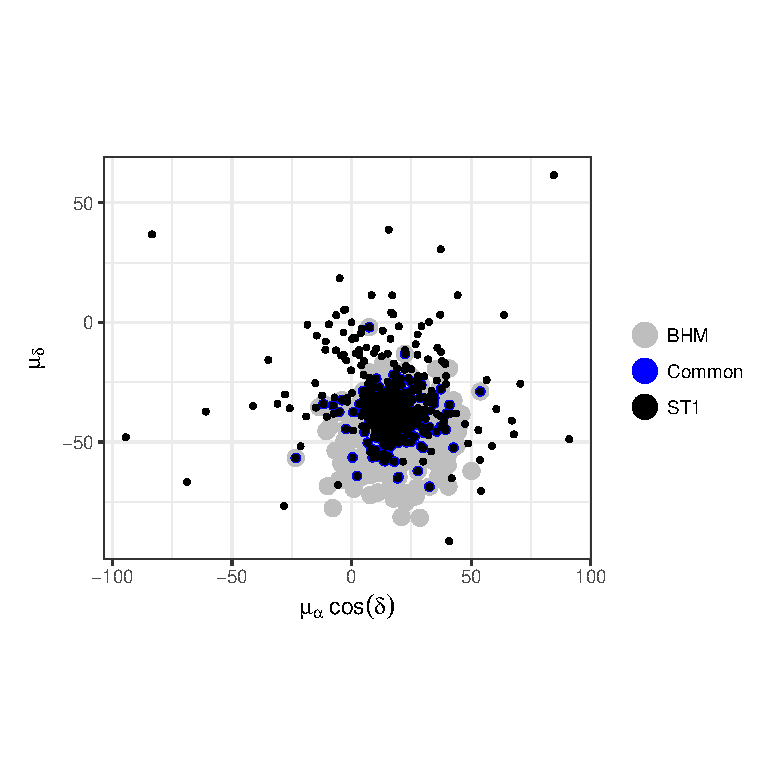
\includegraphics[width=\textwidth]{background/Figures/ST1_pm.eps}
        \caption{}
    \end{subfigure}
    \begin{subfigure}[t]{0.45\textwidth}
    \centering
     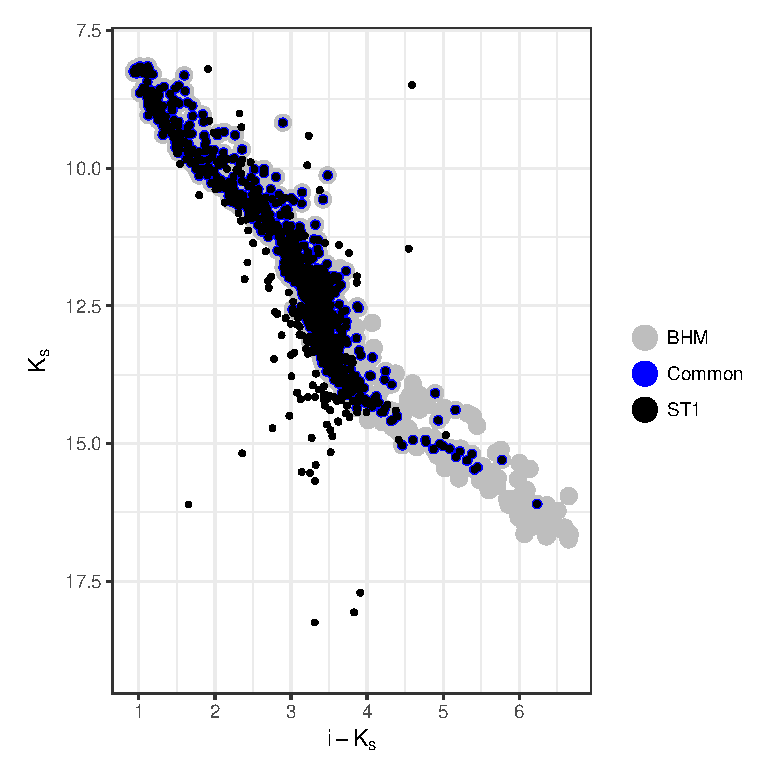
\includegraphics[width=\textwidth]{background/Figures/ST1_ph.eps}
        \caption{}
    \end{subfigure}
\caption{Proper motions (a) and $K$ vs $i-K$ CMD (b) of the ST1 candidate members in the DANCe DR2 catalogue (black). Also shown, the objects classified as candidate members  in the BHM (grey), and in both ST1 and BHM (blue).}
\label{fig:ST1}
\end{figure}

\begin{figure}[ht!]
    \centering
    \begin{subfigure}[t]{0.45\textwidth}
    \centering
       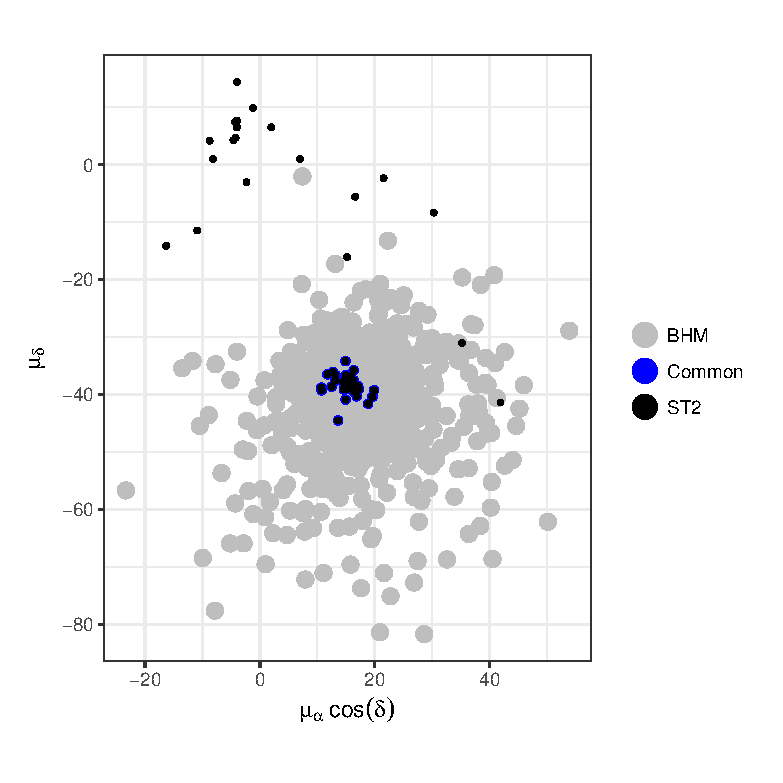
\includegraphics[width=\textwidth]{background/Figures/ST2_pm.eps}
        \caption{}
    \end{subfigure}
    \begin{subfigure}[t]{0.45\textwidth}
    \centering
     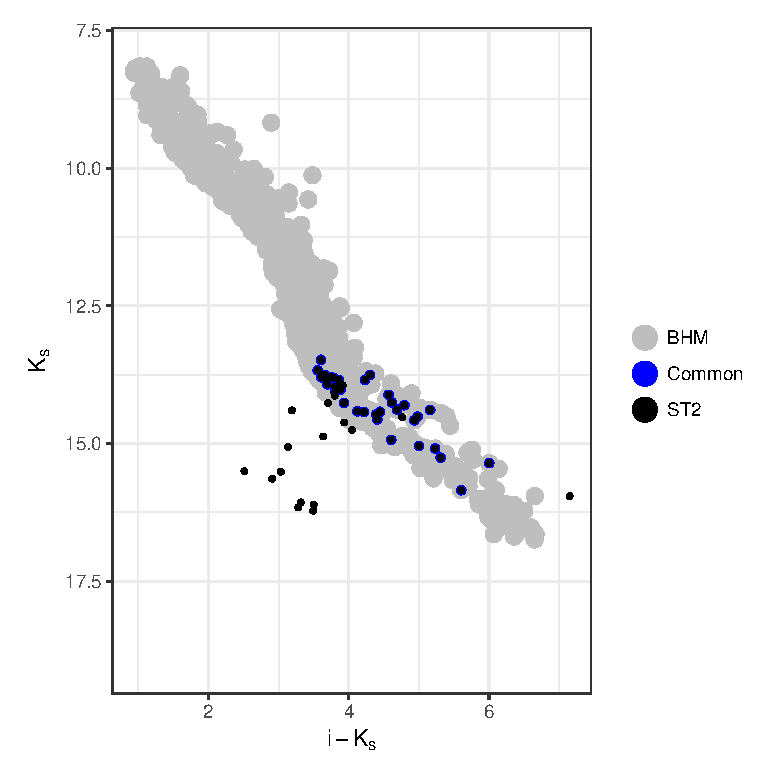
\includegraphics[width=\textwidth]{background/Figures/ST2_ph.eps}
        \caption{}
    \end{subfigure}
\caption{Proper motions (a) and $K$ vs $i-K$ CMD (b) of the ST2 candidate members in the DANCe DR2 catalogue (black). Also shown, the objects classified as candidate members in the BHM (grey), and in  both ST2 and BHM (blue).}
\label{fig:ST2}
\end{figure}

\subsection{Candidate members from \citet{Bouy2015}}
\label{sect:comparisonBouy}

The fact that the work of \citet{Bouy2015} and the present one use the same DANCe DR2 data set (although our model is constructed on the RDR2), allow me to directly compare the membership probabilities of both works. Furthermore, this comparison can be extended to all objects in the data set and not just to the candidate members of the Pleiades cluster. Since \citet{Bouy2015} reported only an statistic of the membership probability distributions, to do a fair comparison, I summarise the membership probability distributions recovered by the BHM with the mode.

Using the optimal probability threshold of 0.84 to classify the cluster members, we can see that, as shown by Fig. \ref{fig:BHMBouy}, both methodologies agree on the outstanding $99.6$\% of the classified objects. Concerning just the candidate members, the agreement is still high, $\sim 90\%$. In the following I discuss the 10\% discrepancies.

\begin{figure}[ht!]
\begin{center}
\resizebox{\textwidth}{!}{\includegraphics{background/Figures/BHM/BHMvsBouy.pdf}}
\caption{Mode of the membership probabilities recovered by the BHM compared to those of \citet{Bouy2015}. The lines show the 0.75 and $p_t=0.84$ probability thresholds used in both works. The numbers indicate our new candidate members (top left), the ones we rejected (bottom right), and the common ones (top right). Reproduced from Figure 11 of \citet{Olivares2017},\textit{\usebibentry{Olivares2017}{title}}, \usebibentry{Olivares2017}{journal}, \usebibentry{Olivares2017}{volume}.}
\label{fig:BHMBouy}
\end{center}
\end{figure}

The candidate members of \citet{Bouy2015} that the BHM rejects, which I call the rejected ones, are shown in lower right box of Fig. \ref{fig:BHMBouy}. They amount to 12\% and 12.5\% of total number of candidate members recovered by \citet{Bouy2015} and the present work, respectively. The 12\% figure is 4.7\% higher than the contamination rate (CR) reported by \citet{Sarro2014} ($7.3\pm1.4$\%). It indicates that some true cluster members must be within the rejected objects. Also, the 12.5\% figure is 2.5\% higher than the 10\% loss rate of the BHM (TPR=90\%, see Section \ref{sect:classifier}), which indicates that some contaminants must be within the rejected objects.

Now, I analyse these objects with further detail. As it is shown in Figs. \ref{fig:rejecteds} and \ref{fig:rejectedsCOLORS}, the rejected objects have proper motions uncertainties with median $\tilde{\mu}_{\alpha},\tilde{\mu}_{\delta}=\{3.15,3.19\} \,\mathrm{mas\cdot yr^{-1}}$. This value is more than four times larger than that of the common candidate members (those objects classified as members by both works, see top right corner of Fig. \ref{fig:BHMBouy}). Among these objects, those with a relatively high membership probability occur mostly at the middle of the cluster photometric sequence (green squares of Fig. \ref{fig:rejectedsCOLORS}). On the other hand, those with lower membership probabilities occur at the bright and faint ends (blue and red triangles of Fig. \ref{fig:rejectedsCOLORS}, respectively). Furthermore, the proper motions uncertainties of the rejected objects at the bright, middle and faint ends of the cluster photometric sequence, have medians of $\tilde{\mu}_{\alpha},\tilde{\mu}_{\delta}=\{4.0,4.2\}  \,\mathrm{mas\cdot yr^{-1}}$, $\tilde{\mu}_{\alpha},\tilde{\mu}_{\delta}=\{2.4,2.4\}\,\mathrm{mas\cdot yr^{-1}}$ and $\tilde{\mu}_{\alpha},\tilde{\mu}_{\delta}=\{3.4,3.4\}\,\mathrm{mas\cdot yr^{-1}}$, respectively. These figures are approximately 6, 4 and 5 times larger, respectively, than those of the candidates in common. These large uncertainties produce a proportional spread of the cluster likelihood. This could reduce the membership probability of these objects.

Furthermore, the bright and faint regions of the cluster photometric sequence coincide with those where objects with missing entries are more frequent (see Fig. \ref{fig:NAsKs}). I stress the fact that the model of \citet{Bouy2015} was constructed using only objects with fully observed vectors of measurements, which represent less than 1\% of the number of objects used by the BHM. Using only fully observed objects, underestimates the field density in the regions where the missing values are more frequent. Underestimating the field likelihood increases the cluster to field likelihood ratio. Therefore it increases also the cluster membership probabilities. This may explain the relatively high membership probabilities reported by \citet{Bouy2015} compared to those of the BHM. In particular, those in the faint region of the photometric cluster sequence. 

Therefore, I consider that both previous phenomena, the large proper motion uncertainties of the rejected objects together with the underestimated field likelihood in \citet{Bouy2015} model, are responsible for the relatively lower BHM membership probabilities of the rejected objects. However, these objects can not be discarded as potential true cluster members. To discard this possibility lower proper motion uncertainties and fewer missing values are needed. Future steps will be taken to try to solve this issue.

 \begin{figure}[ht!]
\begin{center}
\resizebox{\textwidth}{!}{\includegraphics[page=1]{background/Figures/BHM/Rejecteds.pdf}\includegraphics[page=5]{background/Figures/Rejecteds.pdf}}
\caption{Proper motion (left) and $K_s$ vs. $i-K_s$ CMD (right) showing the candidate members of \citet{Bouy2015} rejected by the BHM. Reproduced from Figure 13 of \citet{Olivares2017},\textit{\usebibentry{Olivares2017}{title}}, \usebibentry{Olivares2017}{journal}, \usebibentry{Olivares2017}{volume}.}
\label{fig:rejecteds}
\end{center}
\end{figure}

\begin{figure}[htbp]
\begin{center}
\resizebox{\hsize}{!}{\includegraphics[page=1]{background/Figures/BHM/RejectedsCOLORS.pdf}\includegraphics[page=5]{background/Figures/RejectedsCOLORS.pdf}}
\caption{Proper motion (left) and $K_s$ vs. $i-K_s$ CMD (right)showing the candidate members of \citet{Bouy2015} rejected by the BHM. The colours and shapes are a proxy for their $K_s$ magnitude.Reproduced from Figure 14 of \citet{Olivares2017},\textit{\usebibentry{Olivares2017}{title}}, \usebibentry{Olivares2017}{journal}, \usebibentry{Olivares2017}{volume}.}
\label{fig:rejectedsCOLORS}
\end{center}
\end{figure}

On the other hand, the new candidates members found by the BHM, shown in the upper left box of Fig. \ref{fig:BHMBouy}, amount to 10\% of the \citet{Bouy2015} candidate members. This figure is higher than the $\sim 3.5\%$ of missing rate (1-TPR) reported by \citet{Sarro2014}. Also, these new candidates amount to 9.6\% of the BHM recovered candidate members. This value is larger than the 4.3\% CR reported in Section \ref{sect:classifier}. These two larger figures may indicate that some truly new discoveries may be within these list of new candidate members. In Figs. \ref{fig:newones} I show the proper motions and $K_s$ vs $i-K_s$ CMD of these new candidates members.

The new candidate members have proper motions uncertainties whose median, $\tilde{\mu}_{\alpha},\tilde{\mu}_{\delta}=\{1.33,1.33\} \,\mathrm{mas\cdot yr^{-1}}$, is two times larger than those of the candidate members in common with \citet{Bouy2015}, which have median $\tilde{\mu}_{\alpha},\tilde{\mu}_{\delta}=\{0.65,0.65\} \,\mathrm{mas\cdot yr^{-1}}$. Also, as shown by Fig. \ref{fig:newones}, the majority of the new candidate members, 148, have probabilities lower than 0.95, are located in a halo around the locus of the cluster proper motions, and on top of the cluster photometric sequence in the $K_s$ vs $i-K_s$ CMD. On the contrary, the new candidate members with probabilities higher than 0.95, which are 39, lie in the centre of the cluster proper motions and fall above the cluster sequence in the $K_s$ vs $i-K_s$ CMD. Thus, I hypothesise that: i) Objects whose photometry is compatible with the cluster sequence but are in the proper motions halo, have higher membership probabilities in our methodology due to the increased flexibility of the cluster proper motions model: it now has four gaussians instead of the two of \citet{Bouy2015}. And ii) objects near the centre of the cluster proper motions but located above the cluster photometric sequence sequence, are multiple systems \cite[probably triple systems which can amount to 4\% of the population][]{Duquennoy1991} with an increased membership probability due to our more flexible photometric model of the cluster and equal-mass binaries sequences.

 \begin{figure}[ht]
\begin{center}
\resizebox{\hsize}{!}{\includegraphics[page=1]{background/Figures/BHM/NewOnes.pdf}\includegraphics[page=5]{background/Figures/NewOnes.pdf}}
\caption{Proper motion (left) and $K_s$ vs. $i-K_s$ CMD (right) showing the new candidate members found in this work. Reproduced from Figure 12 of \citet{Olivares2017},\textit{\usebibentry{Olivares2017}{title}}, \usebibentry{Olivares2017}{journal}, \usebibentry{Olivares2017}{volume}.}
\label{fig:newones}
\end{center}
\end{figure}


Summarising, the discrepancies between the BHM membership probabilities and those reported by \citet{Bouy2015} arise from subtle but important differences. The first difference is the treatment of object with missing entries. Although  \citet{Bouy2015} report membership probabilities for this kind of objects, their field and cluster models were constructed discarding them. This may have biased their results. Taking into account objects with missing entries has two consequences. First, the photometric model is more accurate than any other model that discards objects with missing entries. This effect is important in the regions where these objects are more frequent. Second, the use of objects with missing entries in the construction of the cluster model allow us to include the information of good candidate members that were otherwise discarded a priori. A second difference with the model of \citet{Bouy2015}, is the higher flexibility of our cluster model. It allows us to increase the membership probability of the previously discarded candidates. 

\subsection{Candidate members from \citet{Rebull2016}}
\label{sect:comparisonRebull}

After cross matching (at CDS with a 0.5 arcsec radius) the list of candidate members from \citet{Rebull2016} (their Table 2, here after RT1) with the DANCe DR2, I find that 758 out of the 759 objects have a counter part in the DANCE DR2 catalogue. The 91\% of these objects (690 of them) are candidate members in the BHM. Under the assumption that the candidate members in RT1 are indeed true members, which may not be true, the ratio of recovered members is even better than the $TPR=90\pm0.2\%$ reported in Section \ref{sect:classifier}. These objects are shown in Fig. \ref{fig:RT1}.

\begin{figure}[ht!]
    \centering
    \begin{subfigure}[t]{0.45\textwidth}
    \centering
       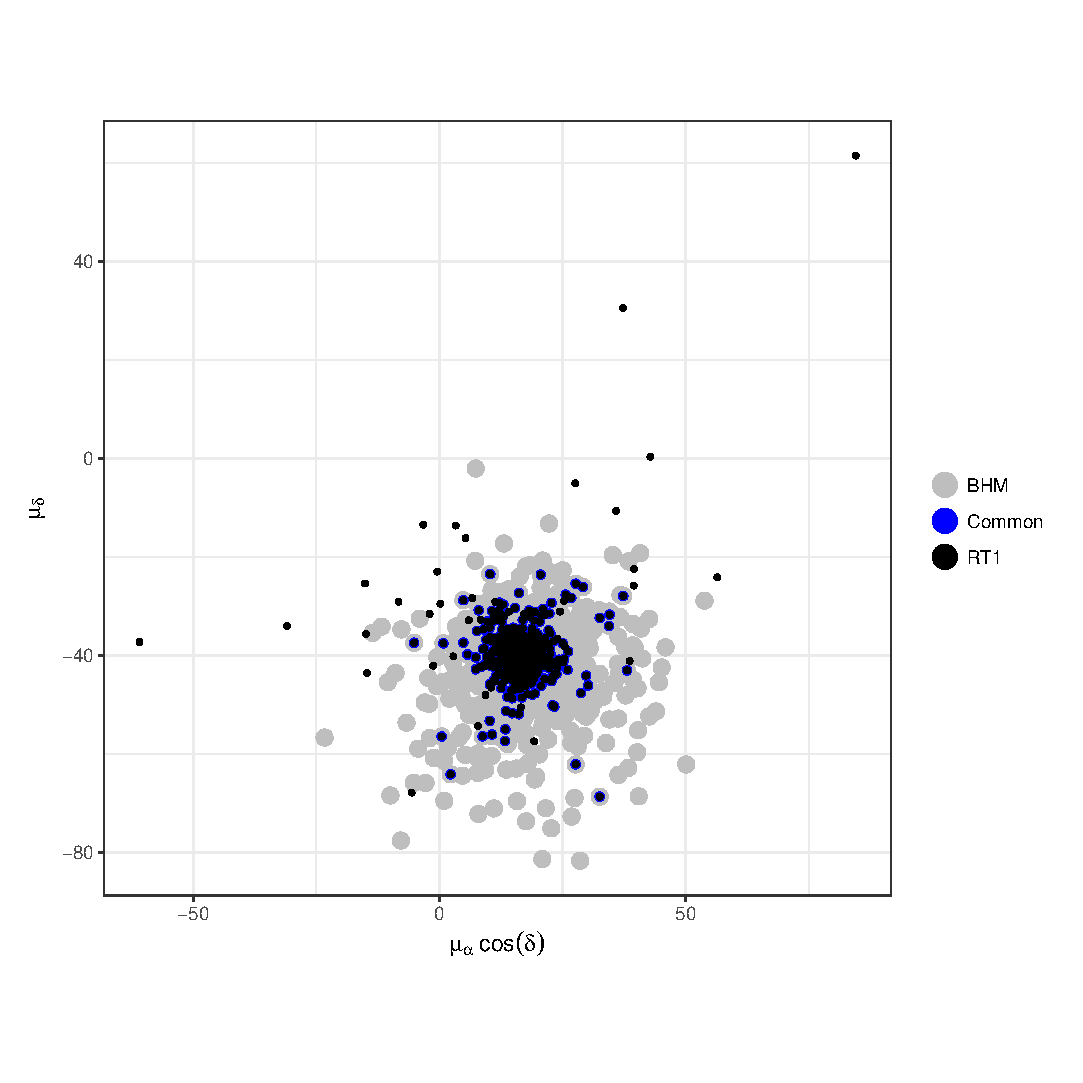
\includegraphics[width=\textwidth]{background/Figures/RT1_pm.eps}
        \caption{}
    \end{subfigure}
    \begin{subfigure}[t]{0.45\textwidth}
    \centering
     \includegraphics[width=\textwidth]{background/Figures/RT1_ph.eps}
        \caption{}
    \end{subfigure}
\caption{Proper motions (a) and $K$ vs $i-K$ CMD (b) of the RT1 candidate members in the DANCe DR2 catalogue (black). Also shown, the objects classified as candidate members  in the BHM (grey), and in both RT1 and BHM (blue).}
\label{fig:RT1}
\end{figure}

On the other hand, after cross matching (at CDS with a 0.5 arcsec radius)  the list of 154 objects that \citet{Rebull2016} classify as non members (their Table 6, here after RT2) with the DANCe DR2, I find that all these objects have a counter part on the DANCe DR2. The 21\% of objects in the RT2 list (33 of them) were classified as candidate members in the BHM. This is a value five times larger than the CR reported in Section \ref{sect:classifier}(CR=4.3\%). However, we can not assume that the RT2 list comprises only non members. First, this objects were at some point classified as members by other authors \cite[Appendix B of][]{Rebull2016}. Second, not all of these objects have periods \cite[only 20\% according to][]{Rebull2016}. From the 33 objects classified as candidate members by the BHM, only nine of them have periods. It means that for the remaining 24 candidate members, these authors used other criteria to discard them as members. In any case, the high rate of BHM candidate members found in this RT2 list may indicate that the criteria used by \citet{Rebull2016} are too restrictive. As can be seen in Fig. \ref{fig:RT2}, these 33 objects have proper motions and photometric measurements consistent with those of the cluster. In order to clarify the status of these 33 objects, further information is still needed.

\begin{figure}[ht!]
    \centering
    \begin{subfigure}[t]{0.45\textwidth}
    \centering
       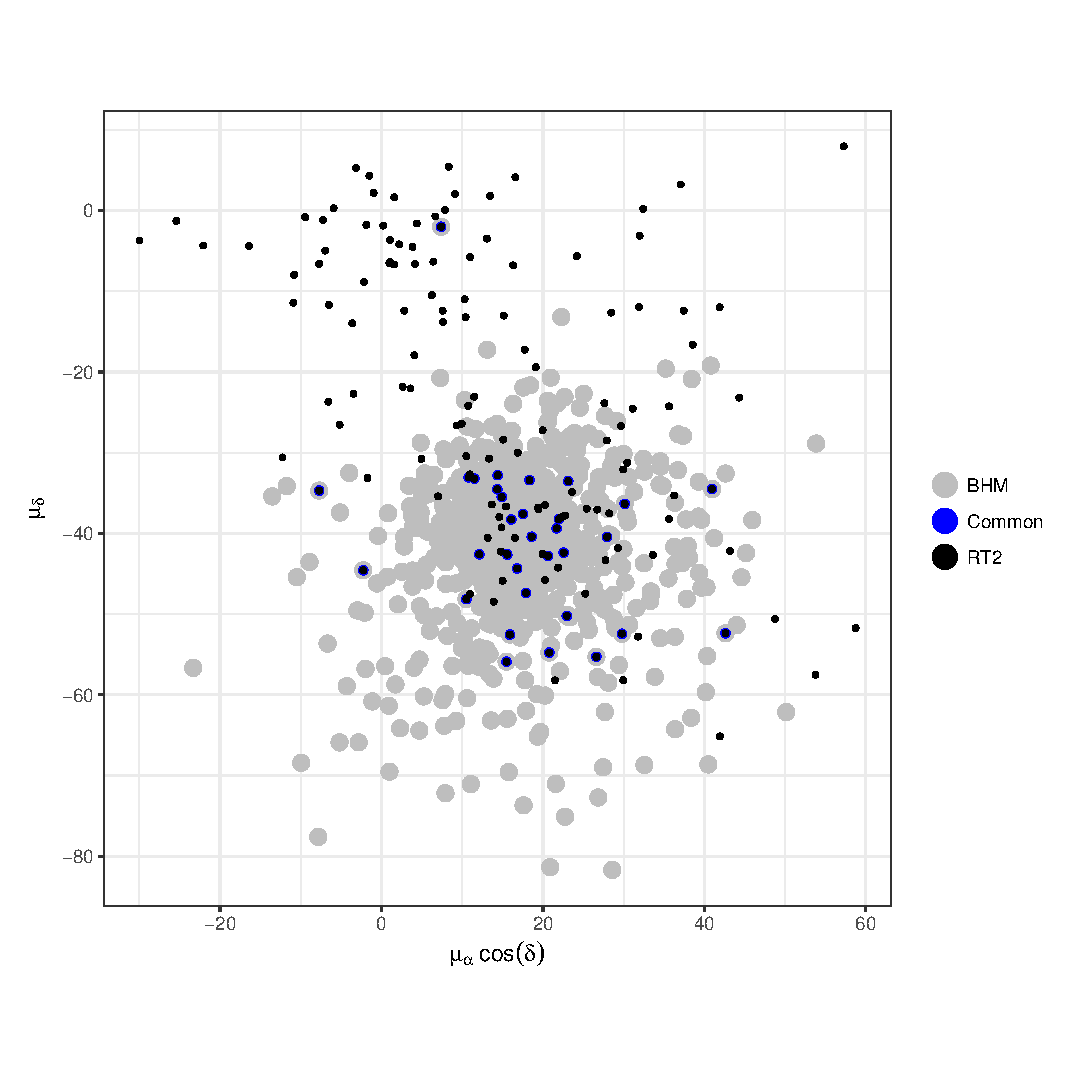
\includegraphics[width=\textwidth]{background/Figures/RT2_pm.eps}
        \caption{}
    \end{subfigure}
    \begin{subfigure}[t]{0.45\textwidth}
    \centering
     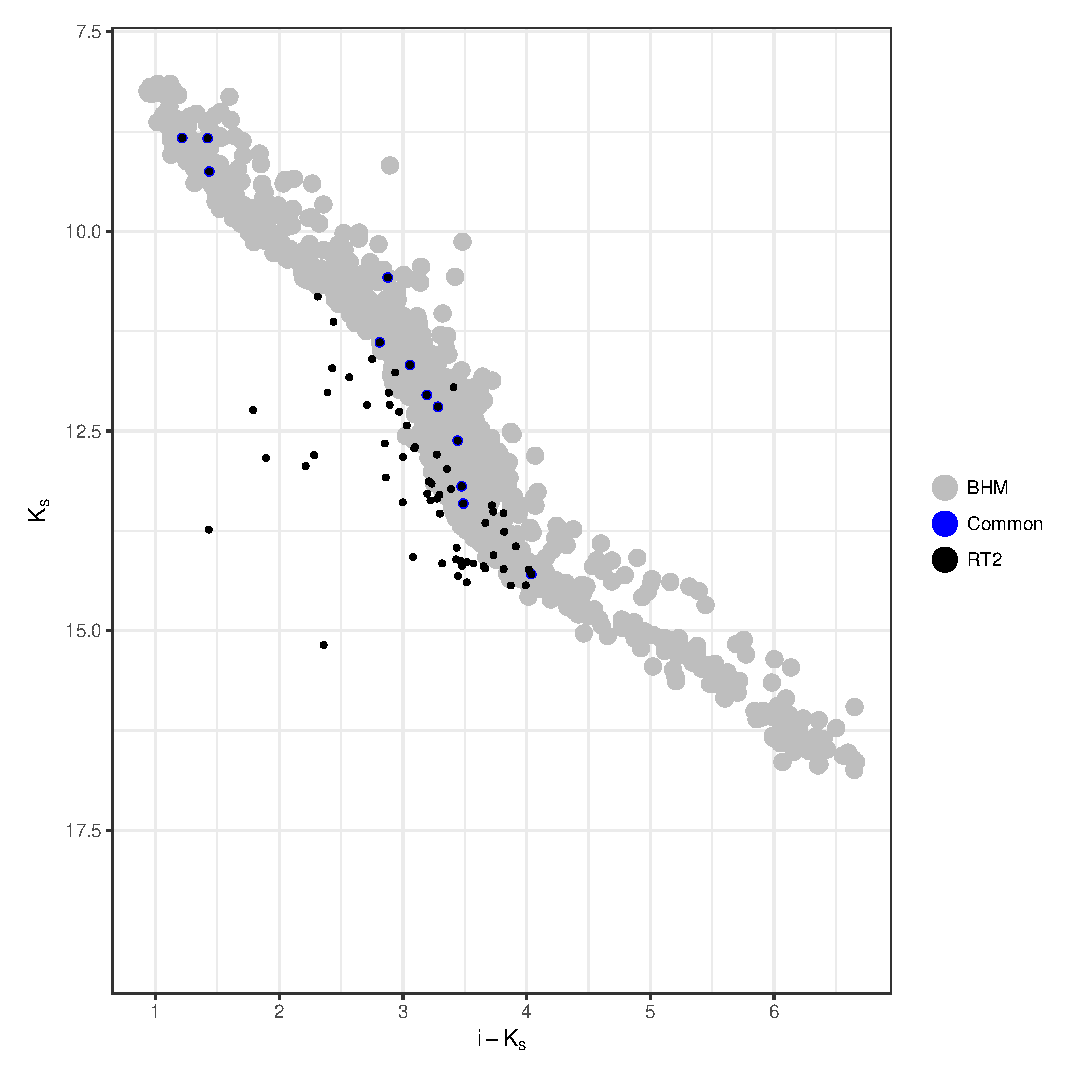
\includegraphics[width=\textwidth]{background/Figures/RT2_ph.eps}
        \caption{}
    \end{subfigure}
\caption{Proper motions (a) and $K$ vs $i-K$ CMD (b) of the RT2 in the DANCe DR2 catalogue (black). Also shown, the objects classified as candidate members in the BHM (grey), and those classified as non members in the RT2 and as candidate members in the BHM (blue).}
\label{fig:RT2}
\end{figure}
 
\section{The statistical distributions of the Pleiades cluster.}
Now, I present the results of the statistical distributions that describe the cluster population, which are the main objective of the present work. These distributions result directly or indirectly from the posterior distribution of the parameters in our model. Indirectly means that I use them as parameters of other function (e.g. the mass distribution). Since we have 85 parameters in the BHM, I only discuss the posterior distributions of some of these parameters. In particular, those related with the velocity, luminosity and mass distributions. Nevertheless, in Table \ref{tab:parameters}, I summarise the posterior distribution of the parameters in our model using the mode, also I use the 16th and 84th percentiles as a proxy for the uncertainty. The parameter names in this Table correspond to those given in Section \ref{sect:priors} (at Table \ref{table:symbols_parameters}). 

Also, for the sake of completeness, in Fig. \ref{fig:correlations} I depict the values the correlation coefficients among the 85 parameters in the BHM. As can be seen from this Figure, the larger correlations appear among parameters describing the true $CI$ distribution, and  among these and almost the rest of the parameters. This is expected since the true $CI$ is key parameter in the BHM. It is also interesting to notice that there is a strong correlation among the coefficients of the splines series modelling different magnitudes. For example, there is a strong correlation among the fourth coefficients of the splines. These correlations are expected since the shape of the cluster sequence is similar in the four CMD.  

\input{background/Tables/TableParameters.txt}

\begin{figure}[ht!]
\begin{center}
\includegraphics[page=1,width=1.1\textwidth]{background/Figures/BHM/Correlations.pdf}
\caption{Correlation matrix of the posterior distributions of the parameters in the BHM. The colour code indicates the value of the correlation coefficient. Parameter names are the same as those in Table \ref{tab:parameters}.}
\label{fig:correlations}
\end{center}
\end{figure}

\section{Updating the prior knowledge}
As mentioned by \citet{Gelman2006}, the posterior distribution must be inspected to update our previous knowledge. To inspect these posterior distribution, I use the statistics reported in Table \ref{tab:parameters}. These values indicate, for example, that the number of  GMM modelling the proper motions of the single stars is overestimated. The fraction and variance of the last gaussian are both to near zero values. Probably, a better model would be that in which the parameters of these extra gaussian will not be part of the model. Ideally, I should choose between these two models based on the evidence they show (see Section \ref{sect:modelselection}). To my knowledge, the only reliable approach to compute the evidence of a model inferred using MCMC, is by means of Nested Sampling (see Section \ref{sect:NestedSampling}). However, running the BHM in the \emph{MultiNest} package lies beyond our current computational resources.

Another example of inspection of the posterior is the following. In a past run of the BHM on the RDR2, I realised that the prior distribution for the parameter modelling field fraction was too narrow. Although the maximum of the posterior distribution was allowed by this prior (by definition), the prior density at this MAP was negligible. Therefore, I updated the prior distribution to a distribution with a larger variance. Thus, I weaken the prior information.
\subsection{Comparing prior values}


\section{Proper motions distribution}
The bivariate proper motions distributions of both single and EMB is directly recovered by the BHM by means of the posterior distributions of the parameters in the GMM modelling these populations.
These bivariate distributions are depicted in Fig, \ref{fig:PM}.

The univariate projections of these distributions, in the $\mu_{\alpha}\cdot cos(\delta)$ and $\mu_{\delta}$ components, are shown in Figs. \ref{fig:PMCs} and \ref{fig:PMBs}. Also, I show in this Figs. the densities in the same proper motions projections of the candidate members of \citet{Bouy2015}, and those found by BHM, which have membership probabilities grater than 0.84. Interestingly, the densities rendered by both samples of members are almost identical. Nevertheless, the density resulting from the sample of the posterior distributions of the parameters in the GMMs, differ from the kernel density estimations of the corresponding populations. This difference results from the distinct populations of the two distributions. The BHM finds the posterior distribution of its parameters using the likelihood of all the objects in the data set. The contribution that individual objects have to the total cluster likelihood can be thought to be proportional to their cluster membership probability. Therefore, the observed difference results from those objects whose cluster membership probability is lower than 0.84. The expected number of cluster members in the probability range 0-0.84 amounts to the non negligible value of $\sim 1100$ objects. These objects contaminate the posterior distribution of the parameters in the BHM with an expected value of 5.3\% (see Section \ref{sect:classifier}). Nevertheless, within them also lies a 10\% of true cluster members (as estimated in Section \ref{sect:classifier}). Discarding these true cluster members from the statistical analysis will render it biased. Instead, we decided to include these 10\% possible true cluster members at the small price of a 5.3\% of contamination.

\begin{figure}[ht!]
\begin{center}
\includegraphics[page=2,width=\textwidth]{background/Figures/BHM/MembersModel.pdf}
\caption{Proper motion distributions recovered by the BHM. The dashed and dot-dashed ellipses represent the mode of 100 samples (orange lines) from the posterior covariance matrices in the cluster and EMB GMMs, respectively. Reproduced from Figure 8 of \citet{Olivares2017},\textit{\usebibentry{Olivares2017}{title}}, \usebibentry{Olivares2017}{journal}, \usebibentry{Olivares2017}{volume}.}
\label{fig:PM}
\end{center}
\end{figure}

\begin{figure}[ht!]
    \centering
    \begin{subfigure}[t]{0.45\textwidth}
    \centering
       \includegraphics[page=2,width=\textwidth]{background/Figures/BHM/Cs_members.pdf}
        \caption{}
    \end{subfigure}
    \begin{subfigure}[t]{0.45\textwidth}
    \centering
     \includegraphics[page=3,width=\textwidth]{background/Figures/BHM/Cs_members.pdf}
        \caption{}
    \end{subfigure}
\caption{Proper motions densities resulting from: a 100 element sample from the posterior distributions of parameters in the GMM modelling the single stars (orange spaghetti lines), the kernel density estimation of the BHM candidate members classified as single stars (those whose cluster membership probability is higher than 0.84 and EMB membership probability is lower than 0.5), and, the kernel density estimation of the candidate members of \citet{Bouy2015} whose photometry lies below the EMB sequence (blue line).}
\label{fig:PMCs}
\end{figure}

\begin{figure}[ht!]
    \centering
    \begin{subfigure}[t]{0.45\textwidth}
    \centering
       \includegraphics[page=2,width=\textwidth]{background/Figures/BHM/Bs_members.pdf}
        \caption{}
    \end{subfigure}
    \begin{subfigure}[t]{0.45\textwidth}
    \centering
     \includegraphics[page=3,width=\textwidth]{background/Figures/BHM/Bs_members.pdf}
        \caption{}
    \end{subfigure}
\caption{Proper motions densities resulting from: a 100 element sample from the posterior distributions of parameters in the GMM modelling the EMB stars (orange spaghetti lines), the kernel density estimation of the BHM candidate members classified as EMB stars (those whose cluster membership probability is higher than 0.84 and EMB membership probability is higher than 0.5), and, the kernel density estimation of the candidate members of \citet{Bouy2015} whose photometry lies near the EMB sequence (blue line).}
\label{fig:PMBs}
\end{figure}

\section{Spatial distribution}
To include
\section{Luminosity distribution}
\label{sect:luminosity}
This Section describes the process to obtain the $J,H$, and $K_s$ absolute magnitude distributions from the posterior distributions of the parameters in the BHM. Later, I compare them to those found by \citet{Bouy2015}, in the $K_s$ band specifically. As in the previous section, I also compare these distributions with those resulting from the kernel density estimates of the candidate members of the BHM.

\subsection{Derivation of the magnitude distributions}
\label{subsect:deriveluminosity}
To derive the $J,H,K_s$ magnitude distributions, I first transform the true $CI$ distribution into the $J,H,K_s$ apparent magnitude distributions. In this transformation, the fractions of EMB must be taken into account. To do this, the magnitude distributions of both single and EMB populations are mixed according to their fractions. In the following paragraphs, I describe the process to obtain the $K_s$ apparent magnitude. This process is similar for the rest of the bands. 

Since we aim at the probability distribution of $K_s$, and it depends on the true $CI$, I use this as a nuisance parameter that I later marginalise. Thus, 

\begin{align}
p(K_s | \boldsymbol{\theta}_c) & = \int p(K_s,CI | \boldsymbol{\theta}_c) \cdot dCI =  \int p(K_s | CI ,\boldsymbol{\theta}_c) \cdot p(CI|\boldsymbol{\theta}_c)\cdot \mathrm{d}CI. \nonumber
\end{align}

The term $p(K_s | CI ,\boldsymbol{\theta}_c)$ represents the probability of $K_s$ given the true $CI$ and the cluster parameters $\boldsymbol{\theta}_c$. It is given by Eq. \ref{eq:lik-seq}. The second term, $p(CI|\boldsymbol{\theta}_c)$ corresponds to the GMM modelling the distribution of the true $CI$, it is given by Eq. \ref{eq:colordist}. 

We include the EMB  distribution with an amplitude equal to their fraction, $1-\pi_{CB}$. Thus,

\begin{align}
p(K_s | \boldsymbol{\theta}_c) & =  \int \left[\pi_{CB}\cdot p_{Cs}(K_s| CI, \boldsymbol{\theta}_c) + (1-\pi_{CB})\cdot p_{Bs}(K_s| CI, \boldsymbol{\theta}_c)\right]\nonumber \\& \cdot p(CI|\boldsymbol{\theta}_c)\cdot \mathrm{d}CI. \nonumber \\
& =   \pi_{CB} \int p_{Cs}(K_s| CI, \boldsymbol{\theta}_c) \cdot p(CI|\boldsymbol{\theta}_c) \mathrm{d}CI \nonumber \\
&+ (1-\pi_{CB})\int p_{Bs}(K_s| CI, \boldsymbol{\theta}_c) \cdot p(CI|\boldsymbol{\theta}_c)\cdot  \mathrm{d}CI. \nonumber \\
\end{align}

In this equation, $Cs$ and $Bs$ are the subindices used to distinguish the probability of $K_s$ under the cluster and EMB photometric models, respectively. These probabilities are defined for the vector of photometric measurements, $\boldsymbol{d}_{ph}$ (see Eq. \ref{eq:lik-seq}). Since we are interested only in the distribution of $K_s$ (by now), we marginalise the rest of the photometric entries,including the observed $CI$ (I use a tilde over the observed quantities). Also, the integration limits must change to those of the truncated true colour distribution ($CI_{min}=0.8, CI_{max}=8$). Hence,

\begin{align}
&p(K_s | \boldsymbol{\theta}_c)  =   \pi_{CB} \int_{CI_{min}}^{CI_{max}}\left[ \left[\sum_{i=1}^5 \pi_{CI,i} \cdot \mathcal{N}_t(CI| \mu_{CI,i},\sigma_{CI,i})\right]\right. \nonumber \\
&\cdot  \left.\int_{\tilde{CI},\tilde{Y},\tilde{J},\tilde{H}}\mathcal{N}(\{\tilde{CI},\tilde{Y},\tilde{J},\tilde{H},K_s\}|\boldsymbol{\mathcal{S}}(CI, \boldsymbol{\beta}),\Sigma_{clus})~\mathrm{d}\tilde{CI}~\mathrm{d}\tilde{Y}~\mathrm{d}\tilde{J}~\mathrm{d}\tilde{H}\right] \cdot \mathrm{d}CI \nonumber \\
& + (1-\pi_{CB}) \int_{CI_{min}}^{CI_{max}}\left[\left[\sum_{i=1}^5 \pi_{CI,i} \cdot \mathcal{N}_t(CI| \mu_{CI,i},\sigma_{CI,i})\right]\right.\nonumber\\
&\cdot \left. \int_{\tilde{CI},\tilde{Y},\tilde{J},\tilde{H}}\mathcal{N}(\{\tilde{CI},\tilde{Y},\tilde{J},\tilde{H},K_s\}|T_{Bs}(\boldsymbol{\mathcal{S}}(CI, \boldsymbol{\beta})),\Sigma_{clus})~\mathrm{d}\tilde{CI}~\mathrm{d}\tilde{Y}~\mathrm{d}\tilde{J}~\mathrm{d}\tilde{H}\right]\cdot \mathrm{d}CI. \nonumber 
\end{align}

The derivations of the $J$ and $H$ magnitude distributions are similar. Since this process takes into account the unresolved EMB and the so called single stars, which in fact could be binaries with low mass ratios, then I call these distributions the apparent system magnitude distributions. 

The previous distributions, together with the parallax and extinction of the cluster, are used to obtain the luminosity distributions, more properly the absolute system magnitude distributions. I assume that the distribution of parallaxes of the Pleiades members is normally distributed with mean, $7.44$ mas, and standard deviation $0.42$ mas \citep{Galli2017}. Then, to obtain the absolute magnitude distributions, I subtract this parallax distribution, by means of a convolution, to the $J,H,K_s$ magnitude distributions. Finally, I deredden the previous distributions employing the canonical value of extinction for the Pleiades: $A_v=0.12$ mag \citep{Guthrie1987}. This last values were transformed into the $J,H,K_s$ extinctions using the extinction law of \citet{Cardelli1989}.

The completeness limits of the derived luminosity distributions are acquired as follows. Since the BHM methodology prescribes the \emph{true} photometric quantities based on the \emph{true} colour index $CI$. Then, the completeness limits of the $CI$ distribution dictate those of the luminosity distributions. 

\citet{Bouy2015} mention that, due to the heterogeneous origins of the DANCe DR2 survey, the spatial coverage and sensitivity of the survey is also not homogeneous. To remedy this issue, they identify a region with complete spatial coverage, the inner three degrees of the cluster (see Fig. \ref{fig:originDANCeDR2}). Then, they restricted their photometric analysis to this spatially complete region. 

Restricting their sample of candidate members to this inner region results in a sample of candidate members that is spatially biased. If any dynamical process has been set on the cluster such that the mass distribution of its members is not uniformly distributed in the space, then an spatial cut in a sample of candidate members will result in a bias on the mass distribution. One of such dynamical process is the mass segregation, which, as suggested by \citet{Adams2001} may have happen in the Pleiades cluster. 

Thus, to avoid such biases, I assume that the UKIDSS survey, which is the most profound from among the contributions to the DANCe DR2 catalogue, provides the homogeneous spatial and sensitivity coverage at faint magnitudes (see Fig. \ref{fig:originDANCeDR2}). This survey thus provides the upper completeness limits, which are essentially those reported in the Appendix A of \citet{Bouy2015}, $i\sim23$ mag and $K_s\sim18$ mag.

Since we are interested in the completeness limits of the $CI$, and this equals $i -K_s$, then its completeness limits are defined by those of $i$ and $K_s$ together. In Fig. \ref{fig:completeness}, I show the $K_s$ and $i$ kernel density estimate computed using all sources in the Pleiades DANCe DR2. As can be seen from this Figure, the point with maximum density, which corresponds to $i=21.4$ mag and $K_s=18.1$ mag, should be used to set the upper completeness limits. Notice that, due to the use of the two dimensional density, the upper completeness limit in $i$ is reduced with respect to that of the univariate $i$ distribution. This density shows a sharp decline at bright magnitudes, probably due to saturation of the detectors. To be conservative, I choose $i=13.2$ mag and $K_s=11.0$ mag as the lower completeness limits.

\begin{figure}[htbp]
\begin{center}
\resizebox{\hsize}{!}{\includegraphics[width=0.8\textwidth]{background/Figures/Density-Kvsi.pdf}}
\caption{Density of all DANCe DR2 sources in $K_s$ and $i$ magnitudes. Lines show the chosen completeness limits, $13.2<i<21.4$ mag and $11<K_s<18.1$ mag. The grey area is considered incomplete. Reproduced from Figure 9 of \citet{Olivares2017},\textit{\usebibentry{Olivares2017}{title}}, \usebibentry{Olivares2017}{journal}, \usebibentry{Olivares2017}{volume}.}
\label{fig:completeness}.
\end{center}
\end{figure}

The $CI$ completeness interval is then defined as that of all the points, along the cluster sequence in the $K_s$ vs. $i-K_s$ CMD, for which $i$ and $K_s$ are bounded by their upper and lower completeness limits, respectively. This results in a completeness interval of  $2.7<CI<5.6$ mag. With it, and the cluster sequence (the splines), I derive the completeness intervals for the $J,H,K_s$ bands. Finally, I transform these intervals to absolute magnitudes and deredden them. 

The luminosity distributions of the $J,H,K_s$ bands, together with their completeness limits are shown in Fig. \ref{fig:Luminosities}. I call them model BHM. For the sake of comparison, I also show the following luminosity distributions. First, the luminosity distributions of objects classified as candidate members in the BHM. I call these the discrete BHM distributions. Also, I plot the luminosity distribution resulting from the candidate members of \citet{Bouy2015}, I call them the discrete Bouy. Since the discrete luminosity distributions, both Bouy and BHM, relay on the magnitudes of the individual candidate members, and many of these objects have missing value entries, then I impute their missing entries using those of the nearest euclidean neighbour. 

The difference between the luminosity distributions derived using the posterior distribution of the parameters in the BHM and discrete BHM distributions, comes as well from the fact that the candidate members are not a random sample of the cluster population. As explained before, the luminosity distributions derived from the parameters in the model take into account all objects proportionally to their cluster membership probability. The discrete BHM uses only the high probability candidate members, thus they may be biased by the probability threshold. In addition, the missing value entries of al the objects in the model BHM distributions are marginalised, while in the discrete B
HM they are imputed.
 
On the other hand, the differences between the discrete distributions, the BHM and that of \citet{Bouy2015}, arise mainly at the bright and faint ends ($K_s\sim 4$ mag and $K_s\sim11$ mag). I hypothesise that the origin of these differences lie in the different list of candidate members. As it has been discussed, the model of \citet{Bouy2015} is constructed only based in fully observed objects. The regions where the objects with missing entries happen more frequently is in the bright and faint regions. Therefore, the observed differences in the luminosity distributions may arise from the incomplete treatment that those authors made of objects with missing entries.

\begin{figure}[htbp]
\begin{center}
\resizebox{\hsize}{!}{\includegraphics[width=0.8\textwidth]{background/Figures/BHM/absolute_JHK-log.pdf}}
\caption{Luminosity distribution of $J,H,K_s$ bands (orange spaghetti lines). Also shown: the regions of incompleteness, and, the luminosity distributions computed from: the candidate members of \citet{Bouy2015} (dot-dashed blue line), and our candidate members, ($p_{84\%}>p_t$, dashed black line). Reproduced from Figure 10 of \citet{Olivares2017},\textit{\usebibentry{Olivares2017}{title}}, \usebibentry{Olivares2017}{journal}, \usebibentry{Olivares2017}{volume}.}
\label{fig:Luminosities}.
\end{center}
\end{figure}

\section{Mass distribution}

In this Section I describe the procedure to transform the luminosities distributions into mass distributions. As any other transformation of probability distributions, it demands the together with the transformation, its derivative (see Section \ref{sect:introprobability}).Once the mass distributions is obtained,  then, I compare it to the Initial Mass Functions (IMFs) of \citet{Chabrier2005} and \citet{Thies2007}. Finally, I conclude this section with the analysis of some simple toy models that can be fitted to the derived mass distribution.

\subsection{The mass-luminosity relation}
\label{sect:mass-luminosity}
The mass-luminosity relation is the non linear transformation that enables us to obtain the mass distribution from the luminosity distributions. Given the values of the upper limits of the luminosity distributions (the faint ends), the mass-luminosity relation relies entirely on the current models of stellar atmospheres. Among the different flavours of theoretical stellar evolution models in the literature (those from the Pisa, Padova, Trieste, Geneva, and Lyon research groups)  we choose the BT-Settl models of \citet{Allard2012}. These models go deeper into the lower masses reaching the planetary mass range thus allowing a complete coverage of our luminosity distributions. The rest of the models stay in the $0.1-10\,\mathrm{M_{\odot}}$ range, with the \emph{PARSEC} models been the ones reaching the $0.1\,\mathrm{M_{\odot}}$ limit \citep{Bressan2012}. 

From the BT-Settle grid I choose the CIFIST2011bc for the 2MASS AB photometric system, 120 Myr and solar metallicity. I choose this photometric system because it covers the dynamic range of the DANCe DR2 survey. The age and metallicity values are the closest, within the grid, to the canonical ones (see Section \ref{sect:generalities}). This grid returns values of the luminosity for certain non uniformly distributed values of the mass. As shown in Eq. \ref{eq:transformdistribution}, the transformation of a probability distribution, in this case the luminosities, into the mass distribution is proportional to the derivative of the transformation, which must be continuos. To avoid the discontinuities in the derivatives produced by the grid, we fit the values from the grid using spline series (see Fig. \ref{fig:splineML}). Then, derivative is obtained from these continuos series (see Fig. \ref{fig:der_splineML}). It is important to notice the following two assumptions. First, I assume that the luminosity distributions in $J,H$ and $K_s$ bands are independent between them, and then I obtain a mass distribution for each one of them. Second, I assume that the transformation from luminosities to masses does not have any associated uncertainty. These assumptions must be taken since the isochrone models do not provide neither uncertainties nor a way to incorporate correlations between the mass distributions of distinct photometric bands. 

Figure \ref{fig:splineML} shows the spline fit to the mass-luminosity relations of the BT-Settl absolute $J,H$ and $K_s$ magnitudes (black points) as a function of the mass. Figure \ref{fig:der_splineML} shows the derivative of mass-luminosity relation. The grey shaded areas represent the incompleteness regions of the DANCe survey (see previous section).

\begin{figure}[ht!]
    \centering
    \begin{subfigure}[t]{0.7\textwidth}
    \centering
       \includegraphics[page=1,width=\textwidth]{background/Figures/FitSpline_AllardModels.pdf}
        \caption{}
        \label{fig:splineML}
    \end{subfigure}
    \begin{subfigure}[t]{0.7\textwidth}
    \centering
     \includegraphics[page=2,width=\textwidth]{background/Figures/FitSpline_AllardModels.pdf}
        \caption{}
        \label{fig:der_splineML}
    \end{subfigure}
\caption{Mass-luminosity relations from the BT-Settl models for the $J, H$ and $K_s$ bands of the 2MASS photometric system (black dots). Also shown, the splines fitted to the previous relations, and the incompleteness regions of the DANCe survey (grey areas). }
\label{fig:ML}
\end{figure}

\subsection{Present day system mass distribution}

The mass distribution is independently obtained for the $J,H,K_s$ luminosity distributions by means of the mass-luminosity relations described in the previous section. Since the luminosity functions of Sect. \ref{sect:luminosity} correspond to the luminosity of systems (single stars unresolved binaries and multiple systems), then, the derived mass function corresponds to the Present Day System Mass Distribution (PDSMD).  Figure \ref{fig:MassDistribution} shows the logarithmic PDSMD ($\xi_L$) for the $J,H,K_s$ bands normalised on the completeness limits of the DANCe survey. The logarithmic representation of the mass distribution is a transformation from the natural variable of mass into the logarithm of 10 scale. It is customary to represent the mass distribution in this scale.

\begin{figure}[htbp]
\begin{center}
\resizebox{\hsize}{!}{\includegraphics[page=1]{background/Figures/BHM/MassDistribution.pdf}}
\caption{Normalised logarithmic PDSMD in $J,H,K_s$ band. Also shown the completeness limits computed in previous section and transformed with the mass-luminosity realtion.}
\label{fig:ModelMassFunction}.
\end{center}
\end{figure}

For the sake of comparison, Figure \ref{fig:ModelMassFunction} shows the PDSMD ($\xi_L$) for the $K_s$ band of the previous Figure, together with the three-slope power-law function of \citet{Bouy2015}, and the Initial Mass Functions (IMF) of \citet{Thies2007} and \citet{Chabrier2005}. The standard uncertainties in \citet{Chabrier2005} IMF are those reported in \citet{Chabrier2003}. 

This Figure shows that the PDSMDs derived from the BHM compare well, at least in the completeness interval, with the one proposed by \citet{Bouy2015}. The discrepancies between these two, above $0.3 \mathrm{M_{\odot}} (-0.5 < \log \mathrm{M/M_{\odot}})$ particularly, may have its origin on the following aspects.

The PDSMF of \citet{Bouy2015} is computed using only their candidate members within the central three degree region of the Pleiades DANCe DR2. First, their list of candidate members is not the same as those found by the BHM. Second, the PDSMD derived from the BHM uses all objects in the data set, not just the high membership probability candidates. Third, as mentioned in Section \ref{sect:luminosity}, the cut to the central three degree region may have biased the derived PDSMF of \citet{Bouy2015}. Therefore, the lack of objects that it shows,  in the mass range $0.3 - 0.7 \mathrm{M_{\odot}}$ ($-0.5 < \log \mathrm{M/M_{\odot}} < -0.2$) particularly, may has it origin in the objects that \citet{Bouy2015} did not included in his analysis: those lying outside the inner three degree region. 

To obtain the power-law model that is shown on Fig. \ref{fig:ModelMassFunction} (as the black solid line), the procedure is the following. 

First, I select three competing models: a log-normal function (like that of \citet{Chabrier2003,Chabrier2005}), and two power-law functions of the form $m^{-\alpha}$ with two and three power-law segments. Second, from a 100 sample distribution of the PDSMD in the $K_s$ band (the ones shown as spaghetti lines in Fig. \ref{fig:ModelMassFunction}) I compute the mean distribution. This is, at each of the 200 points grid spanning the completeness interval, I obtain the mean of the probabilities given by the 100 distributions. With this mean distribution I draw a $10^4$ synthetic sample of masses. Third, using \emph{PyMultiNest}\footnote{A Python wrapper to the \emph{MultiNest} program that uses the Nested Sampling algorithm (see Sect. \ref{sect:NestedSampling})} \citep{Buchner2014}, I infer the parameters of the three models given the masses of the synthetic sample. Table \ref{tab:fitPDSMD} gives the MAP of the parameters in each model together with its evidence (see Sect. \ref{sect:modelselection}). Judging by these evidences, the best model is the two segment power-law. 

The two segment power-law model agrees with the three segment model of \citet{Bouy2015}. However, there are still differences, which are clear at the low and high mass ends particularly. Nevertheless, it is in clear discrepancy with the IMFs of \citet{Chabrier2005},  \cite[$m_c=0.25_{-0.016}^{+0.021}$ and $\sigma=0.55_{-0.01}^{+0.05}$, the uncertainties are those reported by][for single objects]{Chabrier2003} and of \citet{Thies2007}. 

The discrepancy between the IMFs and the PDSMD derived from the BHM and the PDSMF of \citet{Bouy2015} may have its origin on the not yet established uncertainties in the mass-luminosity relation, on dynamical effects associated with age, or in a combination of the previous. In the next section I compare the PDSMD of the Pleiades with that of other younger and older clusters in order to analyse if there is evidence of dynamical effects associated with age.

\begin{table*}[ht!]
\caption{Parameters and evidence of models fitted to the PDSMD}
\begin{center}
\begin{tabular}{lll}
Model&Parameters& Log Evidence\\
\hline
LogNormal&$m_c=0.36\pm0.03$&\\
                 &$\sigma=0.46\pm0.02$ & $18.1 \pm 0.1$\\
\hline
Two Segments &$\alpha_0=-0.11\pm0.06$ \ \ $m \in [0.04,0.22\pm0.01]$ & \\ 
&  $\alpha_1=1.13\pm0.1$ \ \ $m \in [0.22\pm0.01,0.56]$&$2222.7\pm0.4$\\
\hline
Three Segments &$\alpha_0=-0.05\pm0.6$ \ \ $m \in [0.04,0.08\pm0.03]$ & \\
                          &$\alpha_1=-0.1\pm0.1$ \ \ $m \in [0.08\pm0.03,0.22\pm0.01]$ & \\ 
                          &$\alpha_2=1.13\pm0.1$ \ \ $m \in [0.22\pm0.01,0.56]$&$2221.2\pm 0.3$\\
\hline
\end{tabular}
\end{center}
\label{tab:fitPDSMD}
\end{table*}%

However, ending this section, I use the PDSMD to give a lower limit to the mass of the cluster. Since the RDR2 data set  still lacks the very low mass range and most of the high mass range, the mass derived from this PDSMD is only a lower limit to the mass of the cluster. From the PDSMD, the cluster mean mass in the entire mass range is $0.26 \pm 0.006 \mathrm{M_{\odot}}$. Thus, the product of this mean mass with the expected number \footnote{As explained before, the expected number of cluster members is the integral, over the whole range of membership probabilities, of number of objects at each membership probability value.} of cluster members ($3116 \pm 110$), gives the expected mass of the cluster in this mass range. This  value is $807^{+38}_{-29} \mathrm{M_{\odot}}$. 

Finally, I notice that, as mentioned in Sect. \ref{sect:mass-luminosity}, the uncertainties in the mass-luminosity relations are yet to be established. Thus the quoted uncertainties of our mass results are underestimated.

\begin{figure}[htbp]
\begin{center}
\resizebox{\hsize}{!}{\includegraphics[page=1]{background/Figures/BHM/ModelsMassDistribution.pdf}}
\caption{Normalised logarithmic PDSMD in $K_s$ band. Also shown the IMFs of \citet{Chabrier2005} (blue dotted line) and  \citet{Thies2007} (turquoise long-dashed line), and power-law models found here (black solid line, see text) and by \citet{Bouy2015} (blue dashed line).}
\label{fig:ModelMassFunction}.
\end{center}
\end{figure}

\section{The mass distribution on time}
As I mention in the previous section, the observed differences between the present day mass distribution and the initial mass functions may have their origin on the temporal evolution of the cluster population. To test this hypothesis, I compare the Pleiades PDSMD ($\sim125$ Myr) with those of the younger Trapezium ($\sim1$ Myr) and Hyades ($\sim 600$ Myr) PDMD. These can be thought as snapshots of the Pleiades past and future mass distributions.

Although this comparison formally lies beyond the objectives of the present work, nevertheless, it gives an idea of the importance that the PDSMD of other NYOC have in the understanding of the formation and evolution of the mass distribution.

Figure \ref{fig:PDSMDcomparison} shows the PDSMD from the Pleiades, together with those of the Trapezium and Hyades\footnote{Kindly provided by Herv\'e Bouy in a private communication}. These PDSMDs correspond to those of  Fig. 11 of \citet{Bouy2015}. As mentioned by \citet{Bouy2015}, the abundance of low-mass stars and brown dwarfs in the range $0.03 - 0.1\,\mathrm{M_{\odot}}(-1.4 < \log \mathrm{M/M_{\odot}} <-1$) seems to diminish with time. The relative increase of objects in the range $-0.4 < \mathrm{\log M/M_{\odot}} < -0.2$ is an effect of the normalisation\footnote{The interesting alternative of open clusters gaining intermediate mass stars is yet to be explored.}. This effect is consistent with the classical scenario in which low-mass stars and brown dwarfs are ejected as the cluster relaxes.

Since I lack the learned BHM for these two open clusters, the following comparison is made on a frequentist hypothesis testing approach, rather than on the proper Bayesian model selection scheme.

In this hypothesis test, the null hypothesis is that the Hyades and Trapezium PDSMDs came, each of them, from the same distribution than the Pleiades. 

If we want to test the null hypothesis that two distributions come from the same parent distribution, Kolmogorov-Smirnov (KS) and the Anderson-Darling (AD) tests are classical options, with the AD the must robust one. To perform these tests, we must compute certain measures from the two distributions. Then, given the measure, the test distribution returns the probability that the two distributions came from the same parent distribution. Finally, we reject the null hypothesis only if the previous probability is lower than certain probability threshold ($\alpha$), which is usually 0.1, 0.05, or 0.01. 

To perform the KS tests we must obtain the maximum distance between the CDFs of the two distributions. Then, using this distance and the KS distribution, we obtain the probability that the two distributions came from the same parent distribution. If this probability is higher than certain probability threshold ($\alpha$) then the null hypothesis can not be rejected. 

However, the KS test can also be applied in a graphical way. Given the $\alpha$ probability threshold, there is a $d_{\alpha}$ distance for which the KS distribution returns a probability $\alpha$. For $d < d_{\alpha}$ $p_{KS}(d) > \alpha$ and for $d > d_{\alpha}$ $p_{KS}(d) < \alpha$. Therefore, given the CDF of one of the distributions that we want to compare and a probability threshold $\alpha$, the region of distance $d_{\alpha}$ around the CDF depicts the hypothesis test. If the CDF of the other distribution lies entirely within this region, then its maximum distance from the first CDF is less than $d_{\alpha}$. Therefore, its probability is greater than $\alpha$ and the null hypothesis can not be rejected.

\begin{figure}[htp]
\begin{center}
\resizebox{\hsize}{!}{\includegraphics{background/Figures/M45vsM42vsM44.pdf}}
\caption{The PDSMDs of the Pleiades (derived here for $J,H,K_s$ bands), Trapezium, and Hyades (both from \citet{Bouy2015}) clusters. They are normalised in the interval of completeness.}
\label{fig:PDSMDcomparison}.
\end{center}
\end{figure}

\begin{figure}[htp]
\begin{center}
\resizebox{\hsize}{!}{\includegraphics{background/Figures/CDF_comparison.pdf}}
\caption{Cumulative distribution functions (CDF) of the PDSMDs from left panel and that of \citet{Chabrier2005} and \citet{Thies2007} system initial mass function (normalised also in the interval of completeness). The shown Pleiades CDF correspond to the $K_s$ band. The grey area depicts the area in which the CDFs (both Trapezium and Hyades) should lie for the null hypothesis not to be rejected (at $\alpha=0.01$).}
\label{fig:PDSMDtest}.
\end{center}
\end{figure}


Figure \ref{fig:PDSMDtest} shows the cumulative distribution functions (CDFs) of the Trapezium, Pleiades (in $K_s$ band) and Hyades PDSMDs. Also and for comparison, I show the CDFs resulting of \citet{Chabrier2005} and \citet{Thies2007} IMFs. The grey area around the Pleiades CDF depicts the graphical KS hypothesis test in which I choose $\alpha = 0.01$.

Furthermore, since the Kolmogorov-Smirnov test uses only the maximum distance between CDFs, I also applied the more robust Anderson-Darling test. It also rejects the null hypotheses (at $p < 0.004$) that the Trapezium and Hyades PDSMDs and the \citet{Chabrier2005} and \citet{Thies2007} IMFs came from the same parent distribution as the Pleiades PDSMD. 

The previous tests suggest that there is enough evidence for the observed differences among the PDSMDs of these three clusters. Also, they suggest that IMFs of \citet{Chabrier2005} and \citet{Thies2007} are statistically different from the  Pleiades PDSMD.  These observed differences, as mentioned in the previous Section, may have its origin on dynamical effects associated with age and relaxation.

 Nevertheless, to claim for reliable evidence supporting these differences, several issues must be solved. First, the uncertainties in the PDSMD must be properly established. Second, the luminosity distributions must include the uncertainties from the data not just from the poissonian counts. For this, the BHM of these cluster must be computed. Finally, the proper way to compare models is under Bayes' theorem.
 




